\chapter{Электрический ток в металлах}

\section{Свободные носители зарядов в металлах}
    \begin{figure}[b!]
        \center
        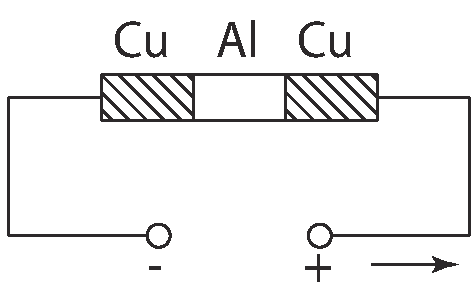
\includegraphics[width=0.47\textwidth]{lec07/rikke.pdf}
        \hfill
        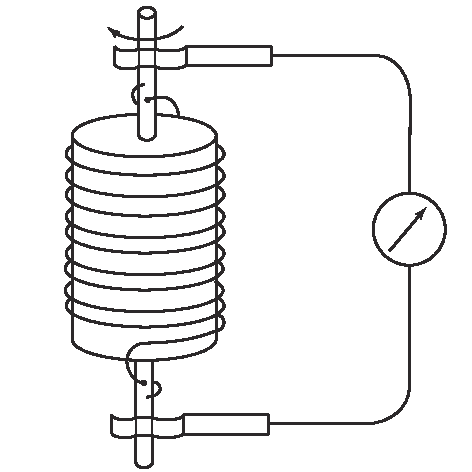
\includegraphics[width=0.47\textwidth]{lec07/tolman.pdf}
        \parbox[t]{.47\textwidth}{\caption{Опыт Рикке}}
        \hfill
        \parbox[t]{.47\textwidth}{\caption{Опыт Толмена-Стюарта}}
    \end{figure}


    \subsection{Опыт Рикке}
        В 1901 году К. Рикке поставил опыт, доказывающий, что в металлах
        носителями свободных зарядов являются не ионы. Для этого он взял три
        цилиндра, два из меди и один из алюминия, и зажав алюминиевый цилиндр
        между медных пропустил через них ток. Если бы носителями были ионы
        кристаллической решётки, то наблюдалось бы видимое проникновение меди в
        алюминий и наоборот. Однако, ничего подобного Рикке не увидел, из чего
        сделал вышеописанный вывод.
    
    \subsection{Опыт Толмена и Стюарта}
        В 1916 году Толменом и Стюартом был поставлен следующий эксперимент:
        катушка с намотанными на нее витками раскручивалась до скоростей
        \( v \sim 300 \text{м}/\text{с} \), а затем резко тормозилась. Через
        баллистический гальванометр проходил импульс тока, переносящий заряд
        \( q \), который и измерялся гальванометром. 
        \[
            q = \int\limits_0^\tau i\dd t,
        \]
        где \( \tau \) -- время торможения. По закону Ома
        \[
            i = \frac{U}{R} = \frac{E_{\textit{ст}}\cdot l}{R},
        \]
        где \( E_{\textit{ст}} \) -- поле сторонних сил, \( l \) -- длина
        проводника. В роли сторонней силы здесь выступает сила инерции:
        \[
            E_{\textit{ст}} = \frac{F_{\textit{инерц}}}{e}.
        \]
        Таким образом,
        \[
            q = \int\limits_0^\tau \frac{F_{\textit{инерц}}\cdot l}{eR}\dd t =
            \frac{l}{eR} \int\limits_0^\tau F_\textit{инерц}\dd t.
        \]
        Интегрируя, получим:
        \[
            q = \frac{l}{eR}\Delta p = \frac{lm}{eR}(v - 0) =
            \frac{m}{e}\frac{lv}{R}.
        \]
        Отсюда следует, что
        \[
            \frac{e}{m} = \frac{lv}{Rq}.
        \]
        Так как справа все величины являются измеряемыми, то это позволило
        Толмену и Стюарту определить удельный заряд носителя
        \[
            \frac{e}{m} \approx 1,7 \cdot 10^{11} \frac{\text{Кл}}{\text{кг}}.
        \]
        А так как отношение заряда электрона к его массе уже было известно, то
        они сделали вывод, что свободными зарядами в металлах являются
        \textit{электроны}.
    
\section{Механизм электрического сопротивления}
    \begin{figure}[!t]
        \center
        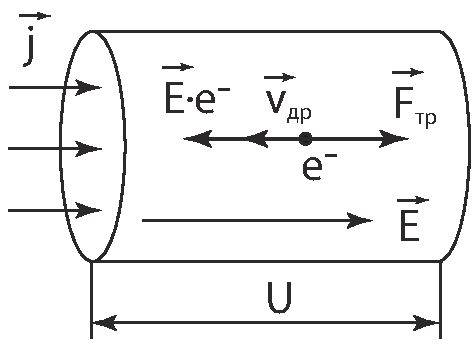
\includegraphics[width=0.47\textwidth]{lec07/resistance_mechanism.pdf} 
        \hfill
        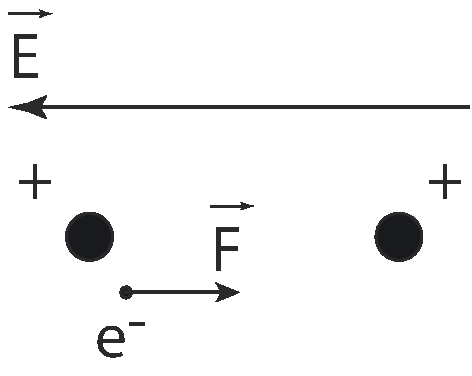
\includegraphics[width=0.47\textwidth]{lec07/classic_theory.pdf}
        \parbox[t]{.47\textwidth}{\caption{Механизм электрического
            сопротивления}}
        \hfill
        \parbox[t]{.47\textwidth}{\caption{Классическая теория металлов}}
    \end{figure}

    На свободные носители зарядов действует сила со стороны поля \( \vec{E} \):
    \[
        \vec{F} = e\vec{E}.
    \]
    А так как, по закону Ома,
    \[
        \vec{j} = \lambda\vec{E} = \frac{1}{\rho}\vec{E},
    \]
    то
    \[
        F = \rho ej = \rho e(nev_{\textit{др}}) = 
        \left(\frac{ne^2}{\lambda}\right)v_{\textit{др}}.
    \]
    
    Таким образом, сила пропорциональна дрейфовой скорости свободных зарядов.
    А так как в конце проводника дрейфовая скорость не растет, то энергия
    переходит в тепло. Следовательно, на свободные носители действует тормозящая
    сила
    \[
        \vec{F}_{\textit{тр}} = -k\vec{v}.
    \]
    
    Природа тормозящей силы -- это неупругие столкновения электронов c ионами
    решетки, в результате которых электроны теряют свой импульс.
    \textit{(см. С.Г. Калашников “Электричество”: \S\S 145 -- 147)}.
   
\section{Классическая теория металлов}
    Основные положения КТМ:
    \begin{enumerate}
    \item свободные носители заряда в металлах -- электроны,
    \item движение электронов описывается законами классической механики,
    \item электроны между собой не взаимодействуют, а взаимодействия с узлами
        решетки являются неупругими.
    \end{enumerate}

    А теперь рассмотрим объяснение уже известных нам законов Ома и Джоуля-Ленца
    с позиций КТМ.
    
\subsection{Закон Ома}

    Пусть \( \tau \) -- это среднее время свободного пробега. И пусть поле
    \( \vec{E} \) не велико, так, что скорость \( v_\textit{max} \) в конце
    свободного пробега много меньше тепловой скорости \( v_\textit{тепл} \sim
    10^5 \text{м}/\text{с} \), то есть \( E \ll 10^8 \text{В}/\text{м} \).
    Поэтому можно считать, что
    \[
        \tau = \frac{\midnum{l}}{v_\textit{тепл}},
    \]
    где \( \midnum{l} \) -- средняя длина свободного пробега.
    
    Тогда, по второму закону Ньютона, приобретенный электроном импульс в конце
    свободного пробега:
    \[
        \Delta p = F\tau = Ee\tau,
    \]
    откуда
    \[
        v_\textit{max} = \frac{\Delta p}{m} = \frac{e}{m}E\tau.
    \]
    
    А так как
    \[
        v_\textit{др} \approx \frac{v_\textit{max}}{2},
    \]
    то
    \[
        v_{\textit{др}} = \frac{e\tau}{2m}E.
    \]
    C учётом \( j = nev_{\textit{др}} \) имеем
    \begin{equation}
        j = \left(n\frac{e^2\tau}{2m}\right)E.
        \label{eq7:1}
    \end{equation}
    
    Сравнивая это с экспериментально установленным соотношением
    \[
        j = \lambda E,
    \]
    получим выражение для \( \lambda \) через микроскопические параметры:
    \begin{equation}
        \lambda = \frac{ne^2\tau}{2m}.
        \label{eq7:2}
    \end{equation}
    
\subsection{Закон Джоуля-Ленца}

    Итак, при неупругом столкновении с узлом решетки электрон отдает ему всю
    накопленную в течение свободного пробега кинетическую энергию, которая
    превращается в тепло:
    \[
        \frac{mv_{\textit{max}}^2}{2} = Q_e.
    \]
    
    Следовательно, если концентрация свободных электронов равна \( n \), то в
    единице объема выделяется тепловая энергия \( w \):
    \[
        w = Q_e\cdot n = \frac{mv_{\textit{max}}^2}{2}n. 
    \]
    Следовательно, в единице объема выделяется тепловая мощность \( p \):
    \[
        p = \frac{w}{\tau} = \frac{mv_{\textit{max}}^2}{2\tau}n.
    \]
    А так как
    \[
        v_{\textit{max}} = \frac{e\tau}{m}E,
    \]
    то
    \begin{equation}
        p = \left(n\frac{e^2\tau}{2m}\right)E^2.
        \label{eq7:3}
    \end{equation}
    С учётом (\ref{eq7:2}), получаем закон Джоуля-Ленца в дифференциальном виде:
    \[
        p = \lambda E^2.
    \]
    
\subsection{Затруднения КТМ}

    \begin{enumerate}
    \item Неверно объясняет температурную зависимость \( \rho \) от температуры
    \( T \). Согласно классической теории
        \[
            \rho = \frac{1}{\lambda}, \, \lambda \sim \tau \Rightarrow \rho \sim 
            \frac{1}{\tau}, \, \tau = \frac{\midnum{l}}{v_{\textit{тепл}}}
            \Rightarrow \rho \sim v_{\textit{тепл}}.
        \]
        А так как
        \[
            \frac{mv_{\textit{тепл}}^2}{2} = \frac{3}{2}kT,
        \]
        то
        \[
            \rho \sim \sqrt{T},
        \]
        тогда как эксперимент дает \( \rho \sim T \).
        
    \item Совершенно не объясняет явление сверхпроводимости: при \( T < 
    T_\textit{крит}\ \rho = 0 \).
        
        \textit{здесь график}
    \end{enumerate}

\section{Границы применимости закона Ома}

    Закон Ома утверждает, что \( i \sim U \). Однако, он совершенно не
    выполняется в следующих случаях:
    \begin{enumerate}
    \item При слишком больших полях \( \vec{E} \sim 10^8 \text{В}/\text{м} \),
        когда время свободного пробега зависит от поля (\( \tau = \tau(E) \)),
        и скорость в конце свободного пробега приближается к тепловой
        \[
            v_{\textit{max}} \approx v_{\textit{тепл}}.
        \]
            
        Тогда, в силу (\ref{eq7:2}), \( \lambda = \lambda(E) \) и
        \( j \nsim E \), а значит не будет и линейной связи между током \( i \)
        и напряжением \( U \).
    
    \item При очень больших частотах \( \omega \gtrsim 10^5 \text{Гц} \)
        (УФ-диапазон).
        
        В этом случае за время колебания \( T \) электрон не успевает пройти
        среднюю длину свободного пробега \( \midnum{l} \), то есть
        \( T < \tau \). Тогда становится бессмысленным понятие времени свобдного
        пробега \( \tau \), а сопротивление среды определяется не столкновениями
        с узлами решетки, а инерционными свойствами электрона.
        
    \item При низких температурах \( T < T_{\textit{крит}} \).
        
        В данном случае \( \rho = 0 \) и, следовательно,
        \( \lambda \rightarrow \infty \).
    
    \item
        Во многих средах:
        \begin{enumerate}
        \item
            в концентрированных электролитах,
        \item
            в газах,
             %(\textit{график с лавинным разрядом})
        \item
            на границе двух полупроводников,
            % ВАХ p-n перехода
        \item
            в вакууме при всех видах эмиссии:
            \begin{enumerate}
            \item
                термоэлектронная эмиссия,
                %-электронная?
            \item
                холодная эмиссия:
                \[
                    j = kE^2 e^{-\frac{\alpha}{E}}.
                \]
                При увеличении \( E \) в 2 раза, ток \( j \) возрастет в
                \( 10^8 \) раз,
            \item
                вторичная эмиссия,
            \item
                фотоэлектронная эмиссия.
                % картинка и ВАХ с током насыщения
            \end{enumerate}
        \end{enumerate}
    \end{enumerate}
